A continuación, se presenta un estimado de las diferentes actividades a desarrollar en el proyecto, con su respectiva duración estimada.

\begin{table}[h]
  \caption{Actividades generales a llevar a cabo}
  \label{tab:Actividades}

  \begin{center}
    \resizebox{14cm}{!}{
      \begin{tabular}{|llll|}
        \hline
        \multicolumn{1}{|c}{Tarea} & \multicolumn{1}{c}{Duración} & \multicolumn{1}{c}{Inicia} & \multicolumn{1}{c|}{Termina} \\ 
        \hline
        \hline
        \multicolumn{1}{|c}{Formalización de la investigación} & \multicolumn{1}{c}{11 Días} & \multicolumn{1}{c}{2 de junio de 2014} & \multicolumn{1}{c|}{14 de junio de 2014} \\ 
        \multicolumn{1}{|c}{Sprint inicial} & \multicolumn{1}{c}{12 Días} & \multicolumn{1}{c}{16 de junio de 2014} & \multicolumn{1}{c|}{1 de julio de 2014} \\ 
        \multicolumn{1}{|c}{Primer Sprint intermedio} & \multicolumn{1}{c}{10 Días} & \multicolumn{1}{c}{2 de julio de 2014} & \multicolumn{1}{c|}{15 de julio de 2014} \\ 
        \multicolumn{1}{|c}{Segundo Sprint intermedio} & \multicolumn{1}{c}{13 Días} & \multicolumn{1}{c}{16 de julio de 2014} & \multicolumn{1}{c|}{1 de agosto de 2014} \\ 
        \multicolumn{1}{|c}{Tercer Sprint intermedio} & \multicolumn{1}{c}{11 Días} & \multicolumn{1}{c}{2 de agosto de 2014} & \multicolumn{1}{c|}{15 de agosto de 2014} \\ 
        \multicolumn{1}{|c}{Cuarto Sprint intermedio} & \multicolumn{1}{c}{12 Días} & \multicolumn{1}{c}{16 de agosto de 2014} & \multicolumn{1}{c|}{1 de septiembre de 2014} \\ 
        \multicolumn{1}{|c}{Quinto Sprint intermedio} & \multicolumn{1}{c}{10 Días} & \multicolumn{1}{c}{2 de septiembre de 2014} & \multicolumn{1}{c|}{15 de septiembre de 2014} \\ 
        \multicolumn{1}{|c}{Sexto Sprint intermedio} & \multicolumn{1}{c}{12 Días} & \multicolumn{1}{c}{16 de septiembre de 2014} & \multicolumn{1}{c|}{1 de octubre de 2014} \\ 
        \multicolumn{1}{|c}{Séptimo Sprint intermedio} & \multicolumn{1}{c}{10 Días} & \multicolumn{1}{c}{2 de octubre de 2014} & \multicolumn{1}{c|}{15 de octubre de 2014} \\ 
        \multicolumn{1}{|c}{Octavo Sprint intermedio} & \multicolumn{1}{c}{13 Días} & \multicolumn{1}{c}{16 de octubre de 2014} & \multicolumn{1}{c|}{1 de noviembre de 2014} \\ 
        \multicolumn{1}{|c}{Noveno Sprint intermedio} & \multicolumn{1}{c}{12 Días} & \multicolumn{1}{c}{2 de noviembre de 2014} & \multicolumn{1}{c|}{15 de noviembre de 2014} \\ 
        \multicolumn{1}{|c}{Sprint final} & \multicolumn{1}{c}{12 Días} & \multicolumn{1}{c}{17 de noviembre de 2014} & \multicolumn{1}{c|}{2 de diciembre de 2014} \\ 
        \hline
      \end{tabular}
      }
      \textbf{Fuente:} Autores
  \end{center}
\end{table}

\begin{figure}
  \begin{center}
    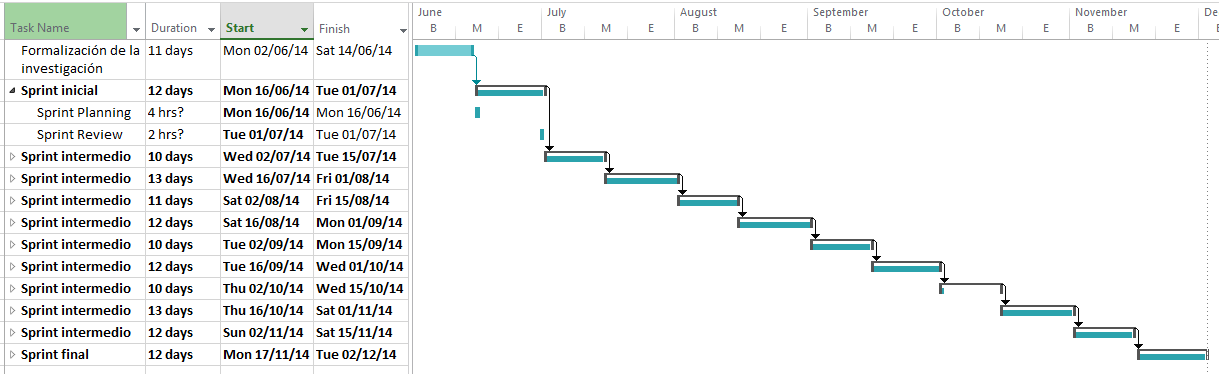
\includegraphics[angle=90,height=18cm,width=8cm]{./imagenes/cronograma_completo.PNG}
    \caption{Distribución de las diferentes actividades a realizar}
    \label{fig:cronograma}
    \textbf{Fuente:} Autores
  \end{center}
\end{figure}

Cabe resaltar que al inicio de cada Sprint realiza un Sprint Planning, y al final un Sprint review.
